\documentclass{article}
\usepackage{amsfonts, amsmath, amssymb, amsthm} % Math notations imported
\usepackage{enumitem}
\usepackage{graphicx}
\usepackage{setspace}
\usepackage{indentfirst}
\usepackage[margin=1in]{geometry}
\graphicspath{{./images/}} % Path to images

% \begin{figure}[htb!]
%      \centering
%      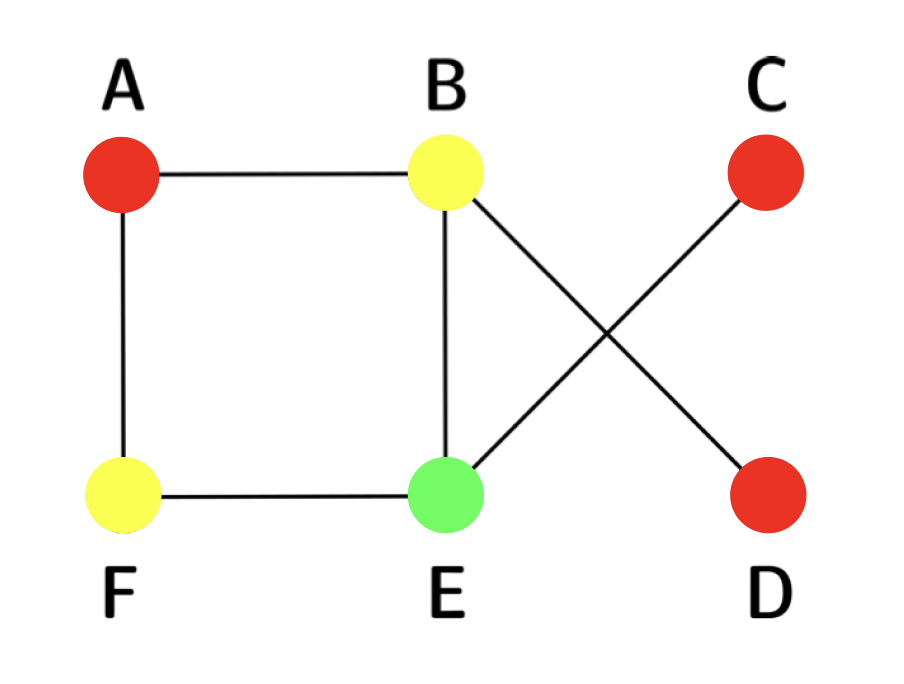
\includegraphics[scale=0.5]{coloring.png}
%      \caption{Coloring of the graph.}
% \end{figure}

% \begin{figure}[htb]
%     \qquad
%     \begin{minipage}{.4\textwidth}
%         \centering
%         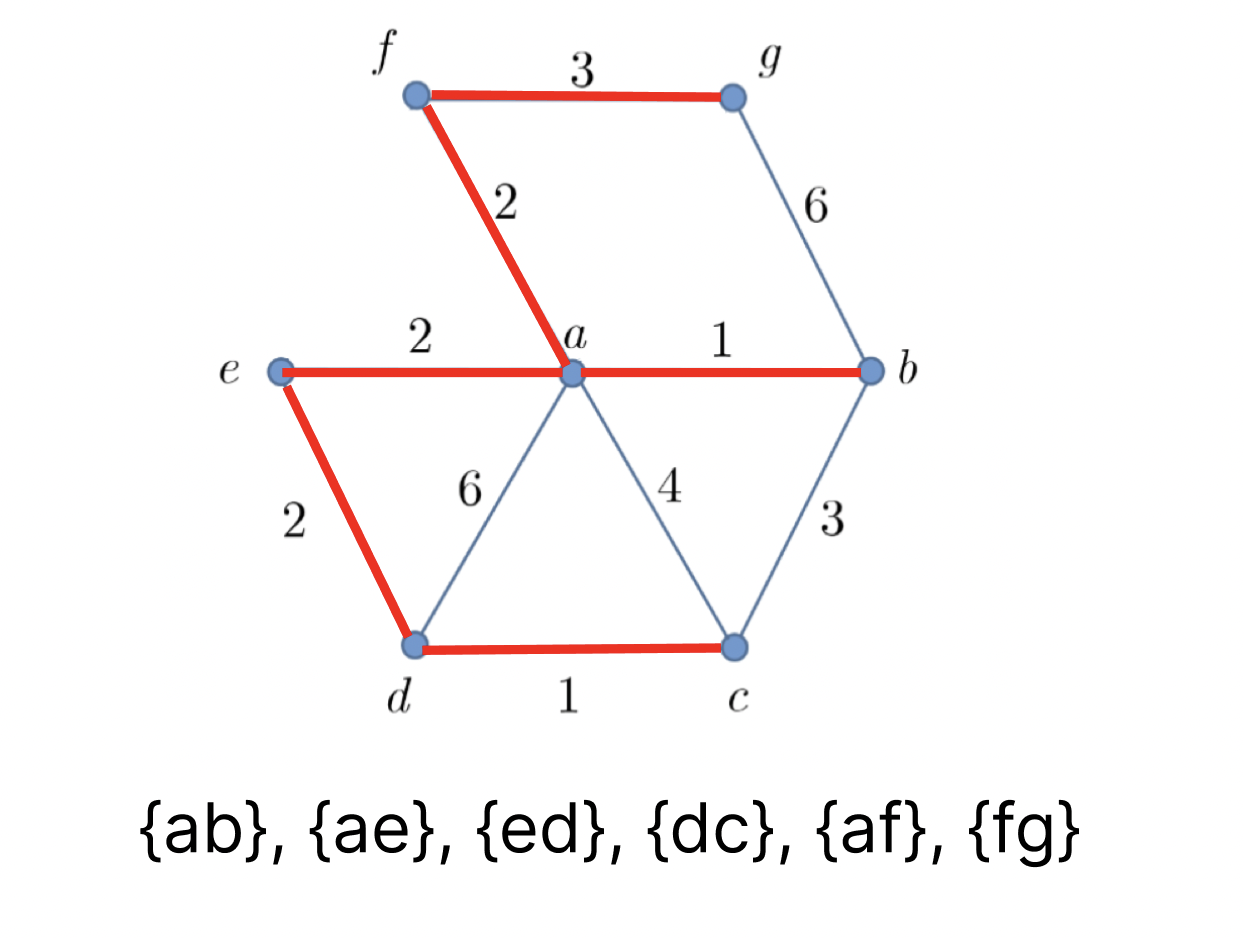
\includegraphics[scale=0.35]{prims.png}
%         \caption{}
%     \end{minipage}    
%     \qquad
%     \begin{minipage}{.4\textwidth}
%         \centering
%         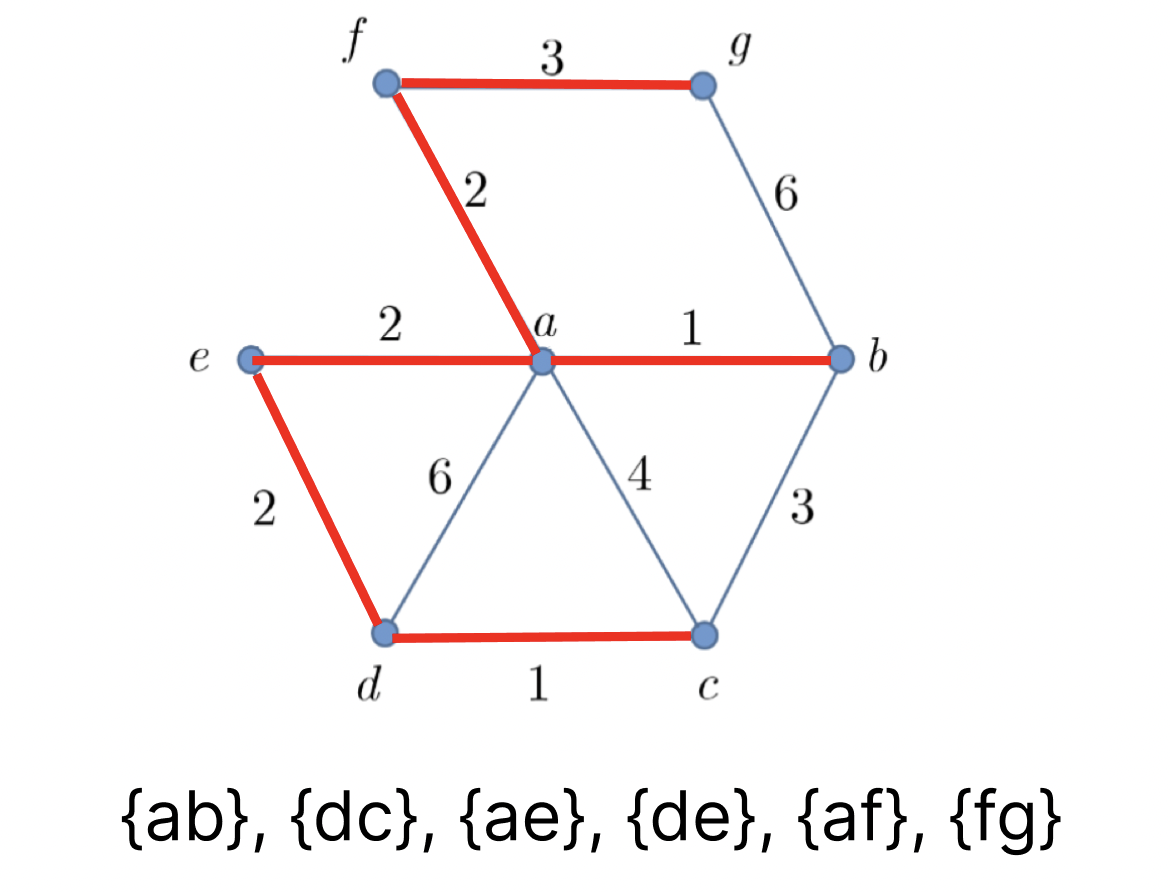
\includegraphics[scale=0.35]{kruskal.png}
%         \caption{}
%     \end{minipage}        
% \end{figure} 

\newtheorem{thm}{Theorem}
\newtheorem{proposition}[thm]{Proposition}
\newtheorem{corollary}[thm]{Corollary}

% title information
\title{Math 104 Practice}
\author{Neo Lee}
\date{2023 Fall}

\setstretch{1.15}
% main content
\begin{document} 

% placing title information; comment out if using fancyhdr
\maketitle 

\section*{Chapter 14}

\begin{proposition}
    $\sum \frac{n^4}{2^n}$ converges.
\end{proposition}
\begin{proof}
    We proceed with Ratio Test.
    \begin{align*}
        \lim\left|\frac{(n+1)^4}{2^{n+1}}\cdot\frac{2^n}{n^4}\right| &= \lim\frac{(n+1)^4}{2n^4} \\
        & = \lim \frac{n^4 + O(n^3)}{2n^4} \\
        & = \frac{1}{2} < 1.
    \end{align*}
\end{proof}

\begin{proposition}
    $\sum\frac{2^n}{n!}$ converges.
\end{proposition}
\begin{proof}
    We proceed with Ratio Test.
    \begin{align*}
        \lim\left|\frac{2^{n+1}}{(n+1)!}\cdot\frac{n!}{2^n}\right| &= \lim\frac{2}{n+1} \\
        & = 0 < 1.
    \end{align*}
\end{proof}

\begin{proposition}
    $\sum\frac{n!}{n^4+3}$ diverges.
\end{proposition}
\begin{proof}
    We proceed with Ratio Test.
    \begin{align*}
        \lim\left|\frac{(n+1)!}{(n+1)^4+3}\cdot\frac{n^4+3}{n!}\right| &= \lim\frac{n(n^4+3)}{(n+1)^4+3} \\
        & = \lim\frac{n^5+3n}{n^4 + O(n^3)} \\
        & = \infty > 1.
    \end{align*}
    Hence, 
    \begin{align*}
        \lim \mathrm{inf}\left|\frac{a_{n+1}}{a_n}\right| =\lim\left|\frac{a_{n+1}}{a_n}\right| =\infty > 1.
    \end{align*}
\end{proof}

\newpage
\begin{proposition}
    $\sum\frac{cos^2n}{n^2}$ converges.
\end{proposition}
\begin{proof}
    We proceed with Comparison Test.
    \begin{align*}
        \left|\frac{cos^2n}{n^2}\right| \le \frac{1}{n^2}.
    \end{align*}
    We know $\sum\frac{1}{n^2}$ converges. Hence, $\sum\frac{cos^2n}{n^2}$ converges.
\end{proof}

\begin{proposition}
    $\sum_{n=2}^{\infty}\frac{1}{log n}$ diverges.
\end{proposition}
\begin{proof}
    We proceed with Comparison Test.
    \begin{align*}
        \frac{1}{log n} \ge \frac{1}{n}.
    \end{align*}
    We know $\sum_{n=2}^\infty\frac{1}{n}$ diverges to $+\infty$. Hence, 
    $\sum_{n=2}^\infty\frac{1}{log n}$ diverges to $+\infty$.
\end{proof}

\begin{proposition}
    Suppose $\sum a_n=A, \sum b_n=B$  where $A, B \in \mathbb{R}$. Then, $\sum (a_n+b_n)=A+B$.
\end{proposition}
\begin{proof}
    Define $(a'_n)$ as the partial sums of $(a_n)$, $(b'_n)$ as the partial sums of $(b_n)$, and 
    $(c'_n)$ as the partial sums of $(a_n+b_n)$. 
    Then
    \begin{align*}
        \sum(a_n+b_n) & = \lim c'_n \\
        & = \lim (a'_n + b'_n) \\
        & = \lim a'_n + \lim b'_n \\
        & = A + B.
    \end{align*}
\end{proof}

\begin{proposition}
    Suppose $\sum a_n=A$  for $A \in \mathbb{R}$. Then, $\sum ka_n=kA$ for 
    $k \in \mathbb{R}$.
\end{proposition}
\begin{proof}
    Define $(a'_n)$ as the partial sums of $(a_n)$ and 
    $(c'_n)$ as the partial sums of $(ka_n)$. 
    Then
    \begin{align*}
        \sum(ka_n) & = \lim c'_n \\
        & = \lim (ka'_n) \\
        & = k\lim a'_n \\
        & = kA.
    \end{align*}
\end{proof}

\begin{proposition}
    Suppose $\sum a_n=A, \sum b_n=B$  where $A, B \in \mathbb{R}$. Then, $\sum (a_n\cdot b_n)=AB$
    is not true in general.
\end{proposition}
\begin{proof}
    Define $(a_n) = (1, 0, 0, 0, \dots), (b_n) = (1/2)^n$. Then $A=1, B=2$ and $AB = 2$. But notice 
    $a_n\cdot b_n = 0$ for all $n\neq 0$ and $\sum(a_n\cdot b_n) = a_0\cdot b_0 = 1\neq AB = 2$.
\end{proof}

\newpage
\begin{proposition}
    If $\sum|a_n|$ converges and $(b_n)$ is a bounded sequence, then $\sum a_nb_n$ converges.
    Note: Corollary 14.7 that absolutely convergent series are convergent is a special case when 
    $(b_n)$ is taken to be 1 for all $n$.
\end{proposition}
\begin{proof}
    Since $(b_n)$ is bounded, we know there exists an supremum for $(|b_n|)$, denote 
    $M = max\{\sup(|b_n|),1\}$. Then, we know there exists $N\in\mathbb{N}$ such that for $n\ge m>N$, 
    $\sum_{k=m}^n|a_k|<\frac{\epsilon}{M}$ for all $\epsilon>0$. Now, take such $N$ and
    \begin{align*}
        \sum_{k=m}^n|a_k| & < \frac{\epsilon}{M} \\
        M\sum_{k=m}^{n}|a_k| & < \epsilon \\
        \left|\sum_{k=m}^{n}a_kb_k\right| \le \sum_{k=m}^{n}|a_k||b_k| \le \sum_{k=m}^{n}|a_k|M & < \epsilon.
    \end{align*}
    Hence, $\sum a_nb_n$ satifies the Cauchy criterion and thus converges.
\end{proof}

\begin{proposition}
    If $\sum a_n$ is a convergent series of nonnegative numbers and $p>1$, then $\sum a^p_n$ 
    converges.
\end{proposition}
\begin{proof}
    We know there exists $N$ such that for $n\ge m>N$, 
    $\left|\sum_{k=m}^{n}a_k\right|<\sqrt[p]{\epsilon}$ for all $\epsilon>0$.
    Take some $\epsilon>0$ and such $N$, then
    \begin{align}
        \left|\sum_{k=m}^{n}a_k\right| & < \sqrt[p]{\epsilon} \nonumber \\
        \left|\sum_{k=m}^{n}a_k\right|^p & < \epsilon \nonumber \\
        \left|\sum_{k=m}^na_k^p\right| \le \left|\left(\sum_{k=m}^na_k\right)^p\right| & < \epsilon.
    \end{align}
    Hence, $\sum a_n^p$ satifies Cauchy criterion and thus converges.

    Note: the left inequality in (1) is true because $a_k\ge 0$ for all $k$ so there are simply extra 
    nonnegative terms in $\left|\left(\sum_{k=m}^na_k\right)^p\right|$.
\end{proof}

\newpage
\begin{proposition}
    If $\sum a_n$ and $\sum b_n$ are convergent series of nonnegative numbers, then 
    $\sum\sqrt{a_nb_n}$ converges. Hint: show $\sqrt{a_nb_n}\le a_n+b_n$ for all $n$.
\end{proposition}
\begin{proof}
    Notice for all $n$
    \begin{align*}
        a_n^2 + b_n^2 + 2a_nb_n & \ge a_nb_n\\
        \left(a_n+b_n\right)^2 & \ge a_nb_n \\
        a_n + b_n & \ge \sqrt{a_nb_n}.
    \end{align*}

    Also, we know there exists $N_1$ such that for $n\ge m>N_1$, 
    $\left|\sum_{k=m}^na_k\right|<\epsilon/2$ and $N_2$ such that for $n\ge m>N_2$, 
    $\left|\sum_{k=m}^nb_k\right|<\epsilon/2$. Now we take $N = \max\{N_1,N_2\}$ for some 
    $\epsilon>0$. Then, for all $n\ge m>N$
    \begin{align*}
        \left|\sum_{k=m}^n\sqrt{a_nb_n}\right| & \le \left|\sum_{k=m}^{n}a_k+b_k\right| \\
        & \le \left|\sum_{k=m}^{n}a_k+\sum_{k=m}^{n}b_k\right| \\
        & \le \left|\sum_{k=m}^{n}a_k\right| + \left|\sum_{k=m}^{n}b_k\right| \\
        & < \epsilon.
    \end{align*}
    Hence, $\sum\sqrt{a_nb_n}$ satisfied Cauchy criterion and thus converges.
\end{proof}

\begin{proposition}
    The convergence of a series does not depend on any finite number of terms, though the 
    value of the limit does. More precisely, consider series $\sum a_n$ and $\sum b_n$ and suppose 
    that the set $\{n\in\mathbb{N}:a_n\neq b_n\}$ is finite. Then the series both converge or else 
    the both diverge.
\end{proposition}
\begin{proof}
    Without loss of generality, we will focus on $\sum a_n$ and conclude the convergence of 
    $\sum b_n$ based on $\sum a_n$. Also, denote $M=\max\{n\in\mathbb{N}:a_n\neq b_n\}$.

    \underline{Case 1: $\sum a_n$ converges.} We know $\sum a_n$ satisfies Cauchy criterion, 
    thus we know there exists $N_1$ such that for all $n\ge m>N_1$, 
    $\left|\sum_{k=m}^{n}a_k\right|<\epsilon$ for some $\epsilon>0$. 
    
    Then, let 
    $N_2=\max\{N_1, M\}$. Since we have set $N_2$ to be at least $M$, any terms after $N_2$ for 
    $b_n$ is the same as $a_n$. Thus, any statement that holds true for $a_n$ is also true for $b_n$
    after $N_2$ and we can conclude for all $n\ge m>N_2$ $\left|\sum_{k=m}^{n}b_k\right|<\epsilon$ 
    for some $\epsilon>0$.

    Therefore, $\sum b_n$ satifies Cauchy criterion too and thus converges.

    \underline{Case 2: $\sum a_n$ diverges.} Assume for the sake of contradiction that $\sum b_n$ 
    converges. Then there exists $N_2$ for all $\epsilon>0$ such that for $n\ge m>N_2$, 
    $\left|\sum b_n\right|<\epsilon$. Thus, we can take $N_1=\max\{N_2,M\}$, which will make sure 
    that for $n\ge m>N_1$, $\left|\sum_{k=m}^n a_n\right|<\epsilon$ for each $\epsilon$. 
    But that contradicts that fact that $\sum a_n$ diverges. Hence, $\sum b_n$ must diverge.
\end{proof}

\begin{proposition}
    Let $(a_n)$ be a sequence of nonzero real numbers such that the sequence 
    $\left(\frac{a_{n+1}}{a_n}\right)$ of ratios is a constance sequence, then $\sum a_n$ is a 
    geometric series.
\end{proposition}
\begin{proof}
    Let $r = \frac{a_{n+1}}{a_n}$ for all $n$. Then we can define $(a_n)$ recursively such that 
    $a_{n+1} = a_n\cdot r$. Hence, $a_n=a_0\cdot r^n$. Indeed, 
    $$\sum a_n = \sum_{k=0}^{n}a_0\cdot r^k,$$ which is a geometric series.
\end{proof}

\begin{proposition}
    Let $(a_n)_{n\in\mathbb{N}}$ be a sequence such that $\lim\inf |a_n|=0$, then there is a 
    subsequence such that $\sum_{k=1}^{\infty}a_{n_k}$ converges.
\end{proposition}
\begin{proof}
    Since $\lim\inf |a_n|=0$, we know there exists a subsequence of $(|a_n|)$ that converges to 0. 
    Hence, for each $\epsilon$, the set $\{n:\mathbb{N}:|a_n|<\epsilon\}$ is infinite. Then 
    we can construct a subsequence such that $\sum_{k=1}^{\infty}a_{n_k}$ converges.

    For each $k+1$, choose $n_{k+1}>n_k$ such that $|a_{n_{k+1}}|<\frac{1}{2^{k+1}}=b_{k+1}$. Then, 
    for each $k$, $|a_{n_k}|\le b_k$. Apparently, $\sum b_k$ is a convergent geometric series, thus 
    by comparison test, $\sum_{k=1}^\infty a_{n_k}$ converges.
\end{proof}

\begin{proposition}
    $\sum_{n=1}^{\infty}\frac{1}{n(n+1)}=1$. Hint: $\sum_{k=1}^{n}\frac{1}{k(k+1)}=
    \sum_{k=1}^{n}\left(\frac{1}{k}-\frac{1}{k+1}\right)$.
\end{proposition}
\begin{proof}
    Notice 
    \begin{align*}
        \sum_{k=1}^{n}\frac{1}{k(k+1)} & = \sum_{k=1}^{n}\left(\frac{1}{k}-\frac{1}{k+1}\right) \\
        & = \left(1-\frac{1}{2}\right) + \left(\frac{1}{2}-\frac{1}{3}\right) + \dots +
        \left(\frac{1}{n}-\frac{1}{n+1}\right) \\
        & = 1 - \frac{1}{n+1}.
    \end{align*}
    Hence, 
    \begin{align*}
        \sum_{n=1}^{\infty}\frac{1}{n(n+1)} & = \lim_{n\to\infty}\sum_{k=1}^{n}\frac{1}{k(k+1)} \\
        & = \lim_{n\to\infty}\left(1 - \frac{1}{n+1}\right) \\
        & = 1.
    \end{align*}
\end{proof}

\begin{proposition}
    $\sum_{n=1}^{\infty}\frac{n-1}{2^{n+1}}=\frac{1}{2}$. 
    Hint: $\frac{k-1}{2^{k+1}}=\frac{k}{2^k}-\frac{k+1}{2^{k+1}}$.
\end{proposition}
\begin{proof}
    Notice 
    \begin{align*}
        \sum_{k=1}^{n}\frac{k-1}{w^{k+1}} & = 
        \sum_{k=1}^{n}\left(\frac{k}{2^k}-\frac{k+1}{2^{k+1}}\right) \\
        & = \left(\frac{1}{2}-\frac{2}{2^2}\right) + \left(\frac{2}{2^2}-\frac{3}{2^3}\right) 
        + \cdots + \left(\frac{n}{2^n}-\frac{n+1}{2^{n+1}}\right) \\
        & = \frac{1}{2} - \frac{n+1}{2^{n+1}}.
    \end{align*}

    Hence, 
    \begin{align*}
        \sum_{n=1}^{\infty}\frac{n-1}{2^{n+1}} & = \lim_{n\to\infty}\sum_{k=1}^{n}\frac{k-1}{2^{k+1}} \\
        & = \lim_{n\to\infty}\left(\frac{1}{2} - \frac{n+1}{2^{n+1}}\right) \\
        & = \frac{1}{2} - \lim_{k\to\infty}\frac{k}{2^k} \\
        & = \frac{1}{2} - \lim_{k\to\infty}\left(\frac{\sqrt[k]{k}}{2}\right)^k \\
        & = \frac{1}{2}.
    \end{align*}
\end{proof}

\begin{proposition}
    Show that $\sum_{n=1}^{\infty}\frac{1}{n}$ diverges by comparing with the series 
    $\sum_{n=2}^{\infty}a_n$ where $(a_n)$ is the sequence 
    $$(\frac{1}{2},\frac{1}{4},\frac{1}{4},\frac{1}{8},\frac{1}{8},\frac{1}{8},\frac{1}{8}
    ,\frac{1}{16},\frac{1}{16},\frac{1}{16},\frac{1}{16},\frac{1}{16},\frac{1}{16},\frac{1}{16}
    ,\frac{1}{16},\frac{1}{32},\frac{1}{32}, \cdots).$$
    
    Note: this is also known as the Cauchy Condensation Test.
\end{proposition}
\begin{proof}
    We will show that $\sum_{n=2}^{\infty}\frac{1}{n}$ diverges and thus 
    $\sum_{n=1}^{\infty}\frac{1}{n}$, which differs only by the first term.

    Notice for all $2^k< n\le2^{k+1}$, $a_n = \frac{1}{2^{k+1}}\le\frac{1}{n}$. This is true for 
    all $k\in\mathbb{N}$. Hence, $\frac{1}{n}\le a_n$ for all $n$. Now observe within each interval 
    $(2^k,2^{k+1}]$, there are $2^k$ terms. Therefore, $\sum_{n=2^k}^{2^{k+1}}a_n=\frac{1}{2}$ and 
    $\sum_{n=2}^{\infty}a_n = \lim_{k\to\infty}k\left(\frac{1}{2}\right)=\infty$. 

    Hence, by Comparison Test, $\sum_{n=1}^{\infty}\frac{1}{n}$ also diverges.
\end{proof}

\newpage
\section*{Chapter 15}
\begin{proposition}
    $\sum \left[sin\left(\frac{n\pi}{6}\right)\right]^n$ diverges.
\end{proposition}
\begin{proof}
    Notice that when $n = 12k + 3, \left[sin\left(\frac{n\pi}{6}\right)\right]^n = 1$. Hence, 
    the summation never converges.
\end{proof}

\begin{proposition}
    $\sum \left[sin\left(\frac{n\pi}{7}\right)\right]^n$ converges.
\end{proposition}
\begin{proof}
    We will show that the summation converges absolutely, hence converges.

    Notice $\left|sin\left(\frac{n\pi}{7}\right)\right|$ is always between 0 and 1. In fact, it is 
    bounded by above by some $r<1$ such that $\left|sin\left(\frac{n\pi}{7}\right)\right| \le r<1$
    and $\left|sin\left(\frac{n\pi}{7}\right)\right|^n \le r^n<1$. 
    Then by Comparison Test, $\sum\left|sin\left(\frac{n\pi}{7}\right)\right|^n$ converges because 
    $\sum r^n$ converges, which can be shown easily by Ratio Test or Root Test.
\end{proof}

\begin{proposition}
    $\sum_{n=2}^{\infty}\frac{1}{n(\log n)^p}$ converges if and only if $p>1$.
\end{proposition}
\begin{proof}
    We proceed with Integral Test with $f(x)=\frac{1}{x(\log x)^p}$. Notice $f(x)$ is continuous,
    positive, and decreasing for $x\ge 2$. Also, $f(n) = a_n$. Then for $p\neq 1$
    \begin{align}
        \lim_{n\to\infty}\int_{2}^{n}\frac{1}{x(\log x)^p}dx & = 
        \lim_{n\to\infty}\left[\frac{(\log x)^{1-p}}{1-p}\right]_2^n.
    \end{align}
    For $p = 1$, we have 
    \begin{align}
        \lim_{n\to\infty}\int_{2}^{n}\frac{1}{x(\log x)}dx & =
        \lim_{n\to\infty}\left[\log(\log x)\right]_2^n = \infty.
    \end{align}

    Then for $(\Rightarrow)$ direction, we know that if $p=1$, (2) goes to infinity, thus the 
    summation diverges. If $p<1$, (1) goes to infinity, thus the summation diverges again. Hence, 
    forward direction is shown by contrapositive.

    For $(\Leftarrow)$ direction, we know that if $p>1$, (1) converges, thus the summation converges.
\end{proof}

\begin{proposition}
    $\sum_{n=4}^{\infty}\frac{1}{n(\log n)(\log\log n)}$ diverges.
\end{proposition}
\begin{proof}
    We proceed with Integral Test with $f(x)=\frac{1}{x(\log x)(\log\log x)}$. Notice $f(x)$ is 
    decreasing, $f(n) = a_n$, and all $a_n$ are nonnegative. Then
    \begin{align*}
        \lim_{n\to\infty}\int_{4}^{n}\frac{1}{x(\log x)(\log\log x)}dx & = 
        \lim_{n\to\infty}\left[\log(\log(\log x))\right]_4^n = \infty.
    \end{align*}
\end{proof}

\newpage
\begin{proposition}
    $\sum_{n=2}^{\infty}\frac{\log n}{n^2}$ converges.
\end{proposition}
\begin{proof}
    \textbf{Integral Test:} 

    We can integrate $f(x)=\frac{\log x}{x^2}$ to get
    \begin{align*}
        \lim_{n\to\infty}\int_{2}^{n}\frac{\log x}{x^2}dx & = 
        \lim_{n\to\infty}\int_{2}^{n}-(\log x)d\left(\frac{1}{x}\right) \\
        & = \lim_{n\to\infty}\left[-\frac{\log x}{x}\right]_2^n +
        \lim_{n\to\infty}\int_{2}^{n}\frac{1}{x^2}dx \\
        & = \lim_{n\to\infty}\left[-\frac{\log x}{x}\right]_2^n -
        \lim_{n\to\infty}\left[\frac{1}{x}\right]_2^n \\
        & = \frac{1}{2},
    \end{align*}
    and conclude that $\sum_{n=2}^{\infty}\frac{\log n}{n^2}$ converges.

    \textbf{Comparison Test:}

    We know that for $n>N$ where $N$ is some constant, $\sqrt{n} > \log n$. This can be proved by 
    obversing that $\sqrt{n} > \log n$ when $n = 100$, and we see by first derivative that 
    $\sqrt{n}$ has a higher increasing rate than $\log n$ for all $n$. Hence, we can conclude that 
    $\sqrt{n} > \log n$ for all $n\ge 100$.

    Then, we see $\frac{\log n}{n^2} < \frac{1}{n^{3/2}}$ for $n\ge 100$. We know that 
    $\sum \frac{1}{n^{3/2}}$ converges for $p>1$ $\Rightarrow \sum_{100}^{\infty}\frac{1}{n^{3/2}}$
    converges $\Rightarrow \sum_{100}^{\infty}\frac{\log n}{n^2}$ converges $\Rightarrow 
    \sum_{2}^{\infty}\frac{\log n}{n^2}$ converges.
\end{proof}

\begin{proposition}
    If $(a_n)$ is a decreasing sequence of real numbers and if $\sum a_n$ converges, then 
    $\lim na_n=0$.
\end{proposition}
\begin{proof}
    Since $\sum a_n$ converges, we know it satisfies Cauchy criterion. In other words, there exists 
    $N$ such that for $n\ge m>N$, 
    \begin{align*}
        \left|\sum_{k=m}^{n}a_k\right| = \sum_{k=m}^{n}a_k & < \frac{\epsilon}{2}.
    \end{align*}
    Notice $(a_n)$ is a decreasing sequence and $\lim a_n=0$ is a necessary condition for $\sum a_n$ 
    to converge, hence all $a_n$ are non-negative. Therefore, we can remove the absolute value.
    
    In particular, for $m=N+1$,
    \begin{align}
        (n-N)a_n & \le \sum_{k=N+1}^{n}a_k \nonumber \\
        na_n & \le \sum_{k=N+1}^{n}a_k + Na_n.
    \end{align}
    Note that since $(a_n)$ converges to 0 and all $a_n$ are non-negative, we know there exists 
    $N'$ such that
    $$a_n  = |a_n-0| < \frac{\epsilon}{2N}.$$
    Therefore, putting back to (4), as long as $n > \max\{N,N'\}$
    $$|na_n - 0| = na_n \le \sum_{k=N+1}^{n}a_k + Na_n < 
    \frac{\epsilon}{2} + N\frac{\epsilon}{2N} = \epsilon.$$
\end{proof}

\newpage
\section*{Chapter 17}
\begin{proposition}
    $\sqrt{x}$ is continuous on its domain $[0,\infty)$.
\end{proposition}
\begin{proof}
    We consider non-negative sequences $(x_n)$ because any sequence with negative terms would not 
    make sense on $f(x_n)$.
    
    We have to show that if $(x_n)$ converges to some $x_0\in[0, \infty)$, $f(x_n)=\sqrt{x_n}$ 
    converges to $\sqrt{x_0}$. In other words, we seek to find $N$ such that for $\epsilon>0$, as 
    long as $n>N$,
    $$|\sqrt{x_n}-\sqrt{x_0}|<\epsilon.$$
    
    Consider $x_0=0$, since $(x_n)\to 0$, there exists some $N$ such that for $n>N$,
    \begin{align*}
        |x_n| & < \epsilon^2 \\
        \sqrt{|x_n|} & < \epsilon \\
        |\sqrt{x_n}| & < \epsilon.
    \end{align*}
    Therefore, $\sqrt{x}$ is continouous at $x=0$.

    For $x_0>0$, we need to show the existence of $N$ such that for $n>N$,
    \begin{align*}
        |\sqrt{x_n}-\sqrt{x_0}| & < \epsilon \\
        \left|\frac{x_n-x_0}{\sqrt{x_n}+\sqrt{x_0}}\right| & < \epsilon \\
        \left|\frac{x_n-x_0}{\sqrt{x_n}+\sqrt{x_0}}\right| \le 
        \left|\frac{x_n-x_0}{\sqrt{x_0}}\right| & < \epsilon \\
        \left|\frac{x_n-x_0}{\sqrt{x_0}}\right| & < \epsilon \\
        \left|{x_n-x_0}\right| & < \sqrt{x_0}\cdot \epsilon.
    \end{align*}
    Indeed, there exists such $N$ because $(x_n)$ converges to $x_0$.
\end{proof}

\begin{proposition}
    If $m\in \mathbb{N}$, then the function $f(x)=x^m$ is continuous on $\mathbb{R}$.
\end{proposition}
\begin{proof}
    Suppose an arbitrary sequence $(x_n)$ that converges to $x_0\in\mathbb{R}$, then 
    \begin{align*}
        \lim f(x_n) & = \lim x_n^m \\
        & = (\lim x_n)^m \\
        & = x_0^m \\
        & = f(x_0).
    \end{align*}
\end{proof}

\begin{corollary}
    Every polynomial function $p(x)=a_0+a_1x+\cdots+a_nx^n$ is continuous on $\mathbb{R}$.
\end{corollary}
\begin{proof}
    Let $f_k = a_kx^k$ for $k\in[0,n]$.
    We have shown in previous proposition that $x^k$ is continuous for $k\in[1,n]$. Notice $x^0=1$ 
    is continuous on $\mathbb{R}$ apparently because every sequence $(x_n)$ that converges to $1$ 
    will have $(x_n)^0=1$.

    Therefore, $f_k$ is continuous on $\mathbb{R}$ because it's a scalar multiple of a continuous 
    function. Consequently, $p(x)$ is continuous on $\mathbb{R}$ because it's a sum of continuous 
    functions.
\end{proof}

\begin{proposition}
    A rational function is a function $f$ of the form $p/q$ where $p,q$ are polynomial functions. 
    The domain of $f$ is $\{x\in\mathbb{R}:q(x)\neq0\}$. Then every rational function is continuous.
\end{proposition}
\begin{proof}
    From \emph{Corollary 26}, we know every polynomial is continous on $\mathbb{R}$ and of course 
    on $\mathbb{R}\backslash \{x:q(x)=0\}$. Hence $p/q$ is continuous since it's a division of two continuous 
    functions where $q\neq0$.
\end{proof}

\begin{proposition}
    $\min(f,g)=\frac{1}{2}(f+g)-\frac{1}{2}|f-g|$.
\end{proposition}
\begin{proof}
    Assume $f>g$, then 
    \begin{align*}
        \frac{1}{2}(f+g) - \frac{1}{2}|f-g| & = \frac{1}{2}(f+g) - \frac{1}{2}(f-g) \\
        & = g \\
        & = \min(f,g).
    \end{align*}
    Assume $g\ge f$, then
    \begin{align*}
        \frac{1}{2}(f+g) - \frac{1}{2}|f-g| & = \frac{1}{2}(f+g) - \frac{1}{2}(g-f) \\
        & = f \\
        & = \min(f,g).
    \end{align*}
\end{proof}

\begin{proposition}
    $\min(f,g)=-\max(-f,-g)$.
\end{proposition}
\begin{proof}
    \begin{align*}
        \max(f,g) & = \frac{1}{2}(f+g)+\frac{1}{2}|f-g| \\
        \max(-f,-g) & = \frac{1}{2}(-f-g)+\frac{1}{2}|-f+g| \\
        \max(-f,-g) & = - \frac{1}{2}(f+g)+\frac{1}{2}|g-f| \\
        -\max(-f,-g) & = \frac{1}{2}(f+g)-\frac{1}{2}|f-g| \\
        -\max(-f,-g) & = \min(f,g).
    \end{align*}
\end{proof}

\begin{corollary}
    If $f$ and $g$ are continuous at $x_0$ in $\mathbb{R}$, then $\min(f,g)$ is continuous at $x_0$.
\end{corollary}
\begin{proof}
    $f,g\in C^0(x_0)\Rightarrow f+g, f-g \in C^0(x_0)\Rightarrow f+g, |f-g| \in C^0(x_0)
    \Rightarrow \frac{1}{2}(f+g), \frac{1}{2}|f-g| \in C^0(x_0)
    \Rightarrow \frac{1}{2}(f+g)+\frac{1}{2}|f-g| \in C^0(x_0)
    \Rightarrow \min(f,g) \in C^0(x_0)$.
\end{proof}

\begin{proposition}
    $g(x)=x^3$ is continuous on $\mathbb{R}$.
\end{proposition}
\begin{proof}
    Consider arbitrary $c\in\mathbb{R}$. We seek to find $\delta$ such that for $|x-c|<\delta$, 
    $|x^3-c^3|<\epsilon$.

    Let's evaluate $|x^3-c^3|$:
    \begin{align*}
        |x^3-c^3| & = |x-c||x^2+xc+c^2| \\
        & \le |x-c|\left(|x^2|+|xc|+|c^2|\right).
    \end{align*}

    For $|x-c|<1$, then 
    \begin{align*}
        |x^2|+|xc|+|c^2| & < |c+1|^2 + |c+1||c| + |c^2|.
    \end{align*}
    Let $M = |c+1|^2 + |c+1||c| + |c^2|>0$. Hence, let $|x-c|<\delta = \min\{\epsilon/M,1\}$, then
    \begin{align*}
        |x^3-c^3| & < |x-c|M < \frac{\epsilon}{M}M = \epsilon.
    \end{align*}
\end{proof}

\begin{proposition}
    Let $f$ be a continuous real-valued function with domain $(a,b)$. If $f(r)=0$ for each rational 
    number $r$ in $(a,b)$, then $f(x)=0$ for all $x\in(a,b)$.
\end{proposition}
\begin{proof}
    We will show that if there are some $x_0\in(a,b)$ such that 
    $f(x_0)=c\neq0$, then $f$ is not continuous at $x_0$, hence not continuous on $(a,b)$.

    Assume for the sake of contradiction that there exists $x_0\in(a,b)\backslash\mathbb{Q}$ such 
    that $f(x_0)=c\neq0$. Let $\epsilon = \frac{|c|}{2}$. However for $|f(x_0)-f(x)|<\epsilon$, there 
    does not exist $\delta$ such that $|x-x_0|<\delta\Rightarrow|f(x_0)-f(x)|<\epsilon$ because 
    there is always a rational number $x'\in (x_0-\delta, x_0+\delta)$ according to the density of 
    $\mathbb{Q}$, and $|f(x')-f(x_0)|=|c|>\epsilon$. Then, the contradiction that $f$ is not 
    continuous is reached.
\end{proof}

\begin{corollary}
    Let $f$ and $g$ be continuous real-valued functions on $(a,b)$ such that $f(r)=g(r)$ for each 
    rational number $r$ in $(a,b)$, then $f(x)=g(x)$ for all $x\in(a,b)$.
\end{corollary}
\begin{proof}
    Let $f(r)=g(r)=c$ and define $f'(x)=f(x)-c$ and $g'(x)=g(x)-c$. Then from \emph{Proposition 33},
    we know $f'(x)=g'(x)=0$ because $f'$ and $g'$ are continuous and $f'(r)=g'(r)=0$. Therefore, 
    $f'(x)=g'(x)=0\Rightarrow f'(x)+c=g'(x)+c=c\Rightarrow f(x)=g(x)=c$ for all $x\in(a,b)$.
\end{proof}

\begin{proposition}
    Let $h(x)=x$ for rational numbers $x$ and $h(x)=0$ for irrational numbers, then $h$ in 
    continuous only at $x=0$.
\end{proposition}
\begin{proof}
    $x_0=0:$ Let $\epsilon>0$. Then for $|x-x_0|<\epsilon$, $|h(x)-h(x_0)|=|h(x)-0|<\epsilon$ because for 
    irrational numbers $x$, $|h(x)-0| = 0<\epsilon$, and for rational numbers $x$, $|h(x)-0|=
    |x-0|<\epsilon$.

    \textbf{$x_0\neq 0$ and irrational}: Let $\epsilon = \frac{|x_0|}{2}$. Assume for the sake of contradiction 
    that there exists $\delta$ such that $|x-x_0|<\delta\Rightarrow|h(x)-0|<\epsilon$. However, 
    by density of $\mathbb{Q}$ there exists a rational number $x'\in (x_0-\delta, x_0+\delta)$ 
    such that $|x'|>|x_0|$ [$x'\in(x_0,x_0+\delta)$ if $x_0>0$, $x'\in(x_0-\delta,x_0)$ if 
    $x_0\le 0$]. Then $|h(x')-0|=|x'|>|x_0|>\epsilon$.

    \textbf{$x_0\neq0$ and rational}: Let $\epsilon = \frac{|x_0|}{2}$. Assume for the sake of contradiction 
    that there exists $\delta$ such that $|x-x_0|<\delta\Rightarrow|h(x)-x_0|<\epsilon$. However, 
    by density of irrationals there exists an irrational number $x'\in (x_0-\delta, x_0+\delta)$. 
    Then $|h(x')-x_0|=|0-x_0|=|x_0|>\epsilon$.
\end{proof}

\begin{proposition}
    For each nonzero rational number $x$, write $x = \frac{p}{q}$ where $p,q$ are integers with 
    no common factors and $q>0$, and then define $f(x)=\frac{1}{q}$. Also define $f(0)=1$ and 
    $f(x)=0$ for all $x\in\mathbb{R}\backslash\mathbb{Q}$. Thus $f(x)=1$ for each integer, 
    $f(\frac{1}{2})=f(\frac{-1}{2})=f\frac{3}{2}=\cdots=\frac{1}{2}$, etc. Then $f$ is continuous 
    at each point of $\mathbb{R}\backslash\mathbb{Q}$ and discontinuous at each point of 
    $\mathbb{Q}$.
\end{proposition}
\begin{proof}
    \textbf{Discontinuous on $\mathbb{Q}$}: Let $x_0\in\mathbb{Q}$. Define a sequence of irrational 
    numbers $(x_n)$ that converges to $x_0$, but $f(x_n)=0$ for all $n$ and obviously $\lim x_n=0\neq
    f(x_0)$ [notice $f(x_0)$ is never 0 for rational number $x_0$].

    \textbf{Continuous on $\mathbb{R}\backslash\mathbb{Q}$}: Let $x_0\in\mathbb{R}\backslash
    \mathbb{Q}$ and $\epsilon>0$. Then let $N=\min\{n>\frac{1}{\epsilon}:n\in\mathbb{N}\}$. 
    Now consider the interval $I = (x_0-1, x_0+1)$. We know there is only a finite number of 
    $\frac{p}{q}\in I$ such that $q<N$ [consider $q=N-1$, there are only finite multiples of 
    $\frac{1}{q}\in I$ because the multiple will eventually "step over" the interval; this is true 
    all for $q<N$]. Since there is only a finite number of such fractions, we can take the fraction 
    that is closest to $x_0$, denote $r$, and let $\delta = |r-x_0|$. Then, the interval 
    $(x_0-\delta,x_0+\delta)$ only contains either irrational numbers or $\frac{p}{q}$ with 
    $q\ge N>\frac{1}{\epsilon}$. 

    Therefore, for rational $x$ such that $|x-x_0|<\delta$, $f(x)\le \frac{1}{N} < \epsilon\Rightarrow
    |f(x)-f(x_0)|=|f(x)-0|<\epsilon$. Obviously for irrational $x$, $|f(x)-f(x_0)|$ is always 0.

    Intuition: We can zoom into $x_0$ to find an interval where only very very small mesh of 
    fractions is contained in there because all larger fractions would "step over" the interval
\end{proof}


\end{document}
